\documentclass[11pt]{article}

% Change "review" to "final" to generate the final (sometimes called camera-ready) version.
% Change to "preprint" to generate a non-anonymous version with page numbers.
\usepackage[final]{acl}

% Standard package includes
\usepackage{times}
\usepackage{latexsym}

% For proper rendering and hyphenation of words containing Latin characters (including in bib files)
\usepackage[T1]{fontenc}
% For Vietnamese characters
% \usepackage[T5]{fontenc}
% See https://www.latex-project.org/help/documentation/encguide.pdf for other character sets

% This assumes your files are encoded as UTF8
\usepackage[utf8]{inputenc}

% This is not strictly necessary, and may be commented out,
% but it will improve the layout of the manuscript,
% and will typically save some space.
\usepackage{microtype}

% This is also not strictly necessary, and may be commented out.
% However, it will improve the aesthetics of text in
% the typewriter font.
\usepackage{inconsolata}

%Including images in your LaTeX document requires adding
%additional package(s)
\usepackage{graphicx}
\usepackage{booktabs}
\usepackage{multirow}
\usepackage{siunitx}
\sisetup{table-format=1.3}

% If the title and author information does not fit in the area allocated, uncomment the following
%
% \setlength\titlebox{5cm}
%
% and set <dim> to something 5cm or larger.

\title{Identifying Large Language Models from Generated Text: A Case Study in Italian Counseling Dialogues}

\author{Simone De Carli \\
  Link\"oping University \\
  % University of Trento \\
  \texttt{simde798@liu.se}
}

\begin{document}
\maketitle

\begin{abstract}
  We investigate whether Large Language Models (LLMs) can be identified from text alone in controlled Italian counseling dialogues. Using TF--IDF $n$-gram representations, unsupervised clustering and linear SVM classification achieve near-perfect separation between four LLMs. Interpretability analysis shows that lexical choices, phrasal patterns, and even personal names contribute to model fingerprints. Simple formatting features alone reach 90\% accuracy, indicating that surface-level cues also reflect model-specific tendencies. These results demonstrate that LLM-generated texts carry distinctive, detectable signatures under identical prompts and dialogue structures.
\end{abstract}

\section{Introduction}

Large Language Models (LLMs) are increasingly deployed as conversational agents across domains. Even under identical prompts and task protocols, different LLMs may exhibit systematic stylistic and linguistic differences. Detecting such differences from generated text alone is relevant for model evaluation, transparency, and attribution.
We investigate whether the underlying LLM used to generate counseling conversations can be identified solely from textual content. We focus on dialogues generated by two virtual agents simulating Brief Action Planning (BAP) counseling sessions, where prompts, language, and interaction structure are held constant across models. This controlled setting allows us to attribute observed variation to model-specific generation behavior.
We combine unsupervised clustering with supervised classification to assess whether structure emerges without labels and to quantify model separability, supported by interpretability analysis identifying characteristic linguistic features.

\section{Theory}

LLM-generated text can be fingerprinted using text mining techniques that capture systematic linguistic patterns. Even with fixed prompts and protocols, different models may exhibit persistent generation biases from architectural choices, training data, and decoding strategies, manifesting as distinctive lexical preferences, phrasal templates, and formatting tendencies.
Authorship attribution research shows that shallow features such as function words, word $n$-grams, and TF--IDF representations effectively distinguish between authors~\cite{unknown}. Similar approaches have been applied to AI-generated text detection, where stylometric representations outperformed simple Bag-of-Words baselines~\cite{kumarage2023stylometricdetectionaigeneratedtext}, suggesting that neural language models leave detectable stylistic signatures.
TF--IDF-weighted word $n$-grams capture these signatures through lexical choice and short-range phrasal patterns. Retaining stop words is important as they encode stylistic rather than semantic information. If model-specific fingerprints exist, texts from different LLMs should form separable groups in this feature space. Unsupervised clustering assesses structure emergence without labels, while supervised classification quantifies separability and enables interpretability through feature weights. Surface-level formatting features may provide complementary signals for model recognition.

\section{Data}

The dataset consists of 1,000 simulated counseling conversations generated for validating a chatbot coach for parents of overweight children, following the Brief Action Planning (BAP) protocol using VALISE~\cite{Bolpagni2025-xw} a tool for simulating dialogues with LLM-based agents. All conversations are in Italian and involve two LLM-based agents as counselor and patient. Prompts and conversational structure are fixed across simulations, with role-playing prompts defining professional BAP counselor and parent roles.
Conversations were generated using four LLMs: \texttt{qwen2.5:32b}, \texttt{qwen2.5:72b}, \texttt{llama3.2-vision:90b}, and \texttt{aya-expanse:32b}, each with five temperature values \{0.1,0.3,0.5,0.7,0.9\}, yielding 50 conversations per model-temperature pair.

Each conversation is treated as a single document by concatenating all dialogue turns.

\section{Method}

We address model recognition using unsupervised and supervised text mining. Each conversation is represented using TF--IDF-weighted bag-of-words over concatenated dialogue turns.
The vectorizer lowercases text, removes numeric characters, and tokenizes on word $n$-grams, retaining stop words as they carry stylistic information. Maximum vocabulary size is fixed at 15,000 terms to ensure equal dimensionality across configurations. We perform grid search over: $n$-gram range (1,2), (1,3), (2,3); minimum document frequency 2, 5; maximum document frequency 90\%, 100\%; sublinear TF scaling enabled, disabled.
$n$-gram ranges exclude unigrams-only (insufficient for stylistic signals) and $n$-grams larger than trigrams (too sparse for the dataset size). Document frequency thresholds filter very rare and common terms that may introduce noise.
To avoid label-dependent bias, we randomly split data into 80\% training and 20\% test sets. Vectorizer parameters are selected exclusively on the training set using $k$-means clustering with silhouette score as the internal metric, without access to ground-truth labels. Once selected, parameters are fixed for all analyses.
$k$-means uses the number of clusters equal to the number of generating models, reflecting our goal of assessing whether texts from different LLMs form distinct groups. The algorithm runs with 10 random initializations to mitigate sensitivity to initial centroids.

After vectorizer tuning, we train a linear SVM in one-vs-rest mode to predict the generating model. Classification performance on the test set quantifies model separability. We validate the method via label shuffling, where randomly permuted labels check for information leakage or artifacts.
We perform margin and weight analysis to identify discriminative features and use a Random Forest classifier with formatting features (newlines, question marks, exclamation marks, character count, word count) to assess whether superficial cues alone enable recognition.
Clustering quality is evaluated post hoc using cluster purity and Adjusted Rand Index (ARI), comparing induced clusters to true labels against a random baseline.

\section{Results}

\subsection{Vectorizer Tuning}

During vectorizer hyperparameter tuning, the best configuration achieved a silhouette score of 0.128 on the training set. This configuration used an $n$-gram range of (1,3), minimum document frequency of 5, maximum document frequency of 100\%, and linear TF scaling (sublinear disabled). Higher-scoring configurations consistently included linear TF scaling and $n$-gram range of (1,3). Lower-scoring configurations tended to use sublinear TF scaling and $n$-gram ranges of (1,2) or (2,3), showing that capturing broader contexts from unigrams to trigrams is important for identifying stylistic patterns, and that sublinear TF scaling may dampen important frequency signals.

We visually inspected clustering results using PCA for dimensionality reduction, as shown in Figure~\ref{fig:best_clusters} (two best configurations by silhouette score) and Figure~\ref{fig:worst_clusters} (worst configuration). The PCA plots show high separation between most clusters, with some overlap between two clusters. Lower silhouette-scoring configurations exhibit slightly more separation between these two clusters and more compact clusters overall. We used PCA because it preserves global structure, making it suitable for assessing overall cluster separation for subsequent linear classification, and because it requires no additional hyperparameter tuning unlike t-SNE or UMAP.\

\begin{figure}[b]
  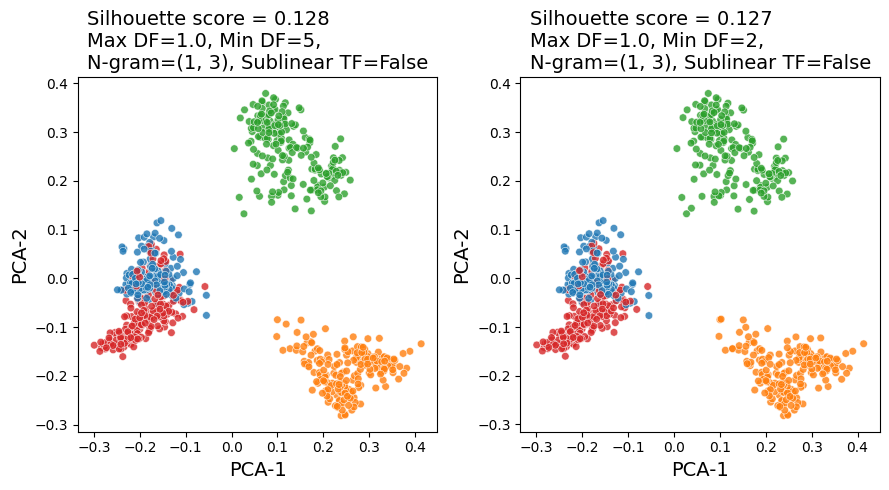
\includegraphics[width=\columnwidth]{images/best_clusters.png}
  \caption{
    PCA projections of the two best clustering configurations according to silhouette score. The first on the left and the second on the right.
  }\label{fig:best_clusters}
\end{figure}

\begin{figure}[t]
  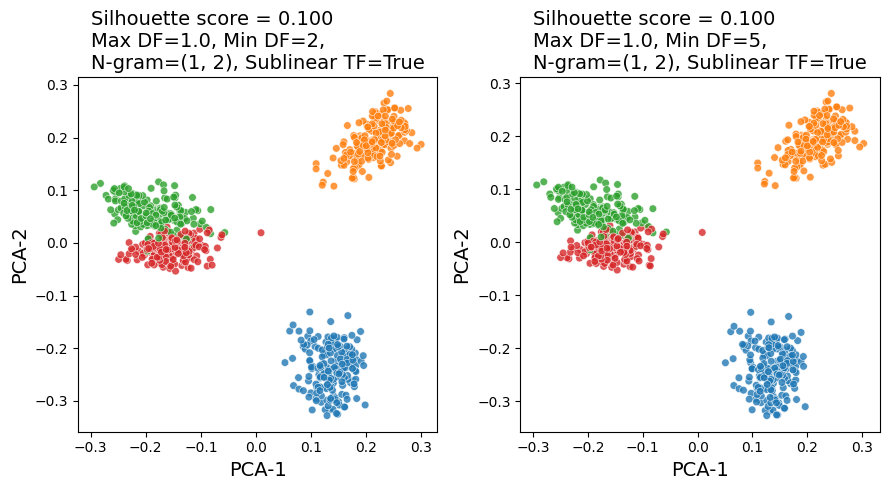
\includegraphics[width=\columnwidth]{images/worst_cluster.png}
  \caption{
    PCA projections of the two worst clustering configuration according to silhouette score. The lowest on the left and the second lowest on the right.
  }\label{fig:worst_clusters}
\end{figure}

\subsection{Clustering Evaluation}

After fixing vectorizer parameters, we evaluated clustering quality on the training set using ARI as an external metric. The best configuration achieved an ARI of 0.997 compared to a random baseline of 0.001, indicating that induced clusters align very closely with true model labels. This suggests that distinct linguistic patterns characteristic of each LLM's generation style are effectively captured by the selected TF--IDF representation.
Cluster purity for each cluster is reported in Table~\ref{tab:cluster_purity}, where each cluster is assigned to its most frequent model. All clusters achieved very high purity: three achieved perfect purity of 1.00, and one achieved 0.99 (one \texttt{aya-expanse:32b} document was assigned to the \texttt{qwen2.5:32b}-dominated cluster).

\begin{table}
  \centering
  \small
  \begin{tabular}{lc}
    \toprule
    \textbf{Model} & \textbf{Purity} \\
    \midrule
    \texttt{aya-expanse:32b} & 1.00 \\
    \texttt{llama3.2-vision:90b} & 1.00 \\
    \texttt{qwen2.5:32b} & 0.99 \\
    \texttt{qwen2.5:72b} & 1.00 \\
    \bottomrule
  \end{tabular}
  \caption{Cluster purity for each cluster where each cluster is assigned to the model that is most frequent in it.}\label{tab:cluster_purity}
\end{table}

We also inspected cluster centroids to identify the most representative terms for each model. The top five terms based on centroid values are reported in Table~\ref{tab:top_terms} with their corresponding TF--IDF values. The identified terms reveal distinctive linguistic patterns and include articles (\emph{di}, \emph{il}, \emph{un}), prepositions (\emph{per}), and common Italian names (\emph{Marco}, \emph{Luca}, \emph{Sofia}, \emph{Alessandro}, \emph{Giovanna}, \emph{Leo}).

\begin{table*}[t]
  \centering
  \small
  \begin{tabular}{ll S S S S S}
    \toprule
    \textbf{Model} &  &
    \textbf{1st} & \textbf{2nd} & \textbf{3rd} & \textbf{4th} & \textbf{5th} \\
    \midrule
    \multirow{2}{*}{\texttt{aya-expanse:32b}}
    & Term   & {di} & {per} & {Leo} & {un} & {Marco} \\
    & TF--IDF & 0.206 & 0.153 & 0.108 & 0.094 & 0.092 \\
    \midrule
    \multirow{2}{*}{\texttt{llama3.2-vision:90b}}
    & Term   & {di} & {per} & {un} & {Alessandro} & {Sofia} \\
    & TF--IDF & 0.192 & 0.133 & 0.095 & 0.094 & 0.093 \\
    \midrule
    \multirow{2}{*}{\texttt{qwen2.5:32b}}
    & Term   & {di} & {per} & {Giovanna} & {il} & {Marco} \\
    & TF--IDF & 0.164 & 0.111 & 0.097 & 0.074 & 0.061 \\
    \midrule
    \multirow{2}{*}{\texttt{qwen2.5:72b}}
    & Term   & {di} & {per} & {Luca} & {un} & {il} \\
    & TF--IDF & 0.165 & 0.116 & 0.112 & 0.083 & 0.076 \\
    \bottomrule
  \end{tabular}
  \caption{Top terms for each model based on cluster centroids, with corresponding TF--IDF weights.}\label{tab:top_terms}
\end{table*}

\subsection{Classification Evaluation}

After fixing vectorizer parameters, we trained a linear SVM classifier on the training set to predict the generating model. On the held-out test set, the classifier achieved 100\% accuracy, indicating perfect separability between texts even with linear decision boundaries. To validate the method, we performed a label shuffling experiment where model labels were randomly permuted before training. The classifier achieved 24\% accuracy, close to the random baseline of 25\%, confirming no information leakage or artifacts were present in the data.
Given perfect classification accuracy, we investigated what made the models so easily separable by analyzing classifier weights for each model. Table~\ref{tab:feature_weights} reports the top five most influential positive and negative features for predicting each model, with their corresponding weights. Again we observe that personal names (\emph{Alessia}, \emph{Giovanni}, \emph{Matteo}, \emph{Piero}) are highly discriminative in favoring or disfavoring certain models. We also observe that 23/40 of the most influential features are unigrams, 12/40 are bigrams, and 5/40 are trigrams, indicating that both individual words and short phrases contribute to model fingerprinting. Frequently there are overlapping words between $n$-grams, indicating that certain roots or stems are particularly characteristic of specific models.

\begin{table*}
  \centering
  \small
  \begin{tabular}{ll l S l S}
    \toprule
    \textbf{Model} & \textbf{Type}
    & \multicolumn{2}{c}{\textbf{Top ($+$)}}
    & \multicolumn{2}{c}{\textbf{Bottom ($-$)}} \\
    \cmidrule(lr){3-4}\cmidrule(lr){5-6}
    & & \textbf{Feature} & \textbf{Weight}
    & \textbf{Feature} & \textbf{Weight} \\
    \midrule

    \multirow{5}{*}{\texttt{aya-expanse:32b}}
    & & Alessia   &  1.1923 & Potresti & -0.6836 \\
    & & più       &  0.6923 & capricci & -0.6457 \\
    & & con il    &  0.6373 & le       & -0.6383 \\
    & & nonni     &  0.6360 & le sue   & -0.6364 \\
    & & il latte  &  0.6359 & sue      & -0.6267 \\
    \midrule

    \multirow{5}{*}{\texttt{llama3.2-vision:90b}}
    & & Ciao          &  0.8487 & Alessia        & -0.7350 \\
    & & venerdì      &  0.7520 & Giovanni       & -0.6602 \\
    & & nella scelta &  0.7482 & una dieta più  & -0.6319 \\
    & & nella        &  0.7412 & dieta più      & -0.6077 \\
    & & scegli per   &  0.6922 & disponibilità  & -0.6040 \\
    \midrule

    \multirow{5}{*}{\texttt{qwen2.5:32b}}
    & & le                     &  0.8802 & pasti              & -0.9818 \\
    & & specifiche puoi fare   &  0.7321 & Matteo             & -0.7074 \\
    & & puoi fare              &  0.6688 & Piero              & -0.6632 \\
    & & puoi fare per          &  0.6575 & Sono qui per       & -0.5900 \\
    & & lei                    &  0.5862 & molto determinato  & -0.5618 \\
    \midrule

    \multirow{5}{*}{\texttt{qwen2.5:72b}}
    & & pasti           &  0.6983 & iniziare     & -0.7159 \\
    & & Sono qui        &  0.6735 & sostegno     & -0.5914 \\
    & & fine settimana  &  0.6553 & momenti      & -0.5480 \\
    & & della famiglia  &  0.6479 & di succo di  & -0.5251 \\
    & & fine            &  0.6042 & di succo     & -0.5212 \\
    \bottomrule
  \end{tabular}

  \caption{Most influential positive (Top) and negative (Bottom) feature weights for each model.}
  \label{tab:feature_weights}
\end{table*}

\subsection{Formatting Features Evaluation}

We evaluated whether superficial formatting cues alone are sufficient for model recognition. We extracted five simple formatting features from the raw text of each conversation: total number of newlines, total number of question marks, total number of exclamation marks, total document length in characters, and total document length in words.
These features capture basic structural aspects that may vary between models. We trained a Random Forest classifier with 50 estimators on the training set using only these formatting features. On the held-out test set, the classifier achieved 90.5\% accuracy, indicating that even superficial formatting cues contain significant information for model recognition. This suggests that different LLMs exhibit distinct tendencies in text structure and punctuation usage, which can be exploited for fingerprinting.

\section{Discussion}

\subsection{Main Findings}

The results demonstrate that LLM-generated texts with fixed prompts and structure can be effectively fingerprinted based on their linguistic patterns alone, even with similar model architectures like the two \texttt{qwen2.5} variants. Both unsupervised clustering and supervised classification achieved near-perfect separability between texts from different models, indicating that distinct generation styles are captured by the TF--IDF representation.
Interpretability analysis revealed that specific words and phrases, including personal names and common Italian articles and prepositions, are highly characteristic of each model's output. This suggests that LLMs may develop unique lexical preferences and stylistic tendencies even when following identical prompts. Additionally, the most influential features of the classifier showed that some models favored or disfavored certain terms or phrases, further highlighting their distinctive generation behaviors.
Personal names appear to play a significant role in model differentiation, possibly reflecting biases of some models toward certain names. Other terms like \emph{pasti} (meals), \emph{latte} (milk), and \emph{capricci} (tantrums) may indicate differing emphases on dietary and behavioral aspects in the counseling context. Phrasings like \emph{puoi fare} (you can do), \emph{nella scelta} (in the choice), and \emph{fine settimana} (weekend) are particularly discriminative, suggesting that certain models may prefer more directive or choice-oriented language. The strong discriminative role of personal names suggests that some fingerprints may stem from prompt-internal name sampling rather than deeper stylistic properties.

\subsection{Formatting Features}

The high classification accuracy achieved using only simple formatting features indicates that superficial text structure also varies systematically between LLMs. Differences in the number of newlines, question marks, and exclamation marks suggest that models may have distinct tendencies in dialogue pacing, interrogative style, and emotional expression. Variations in document length further imply differing verbosity levels that can aid in model recognition. These findings highlight that both deep linguistic patterns and surface-level formatting cues contribute to the fingerprinting of LLM-generated texts. Even though formatting features alone are not sufficient for perfect classification, they provide a strong signal that complements the richer linguistic features captured by TF--IDF representations.

\section{Generalization and Limitations}

While the study demonstrates effective fingerprinting of LLM-generated texts in a controlled counseling dialogue setting, several limitations should be considered. The dataset consists of fixed prompts and structure, which may not be representative of more open-ended or diverse generation scenarios. The analysis is limited to four specific LLMs, and the $k$ parameter of $k$-means was set to the known number of models, which may not generalize to settings with unknown or larger model sets. Additionally, the focus on Italian texts may limit applicability to other languages with different linguistic characteristics, even though the methods are language-agnostic. The interpretability analysis primarily relies on linear model weights, which may not capture more complex interactions between features. Future work could explore more diverse datasets, additional LLM architectures, and advanced interpretability techniques to further validate and extend these findings.

\section{Conclusion}

In this work, we investigated whether Large Language Models can be reliably identified from generated text alone under strictly controlled prompting and interaction conditions. By framing the problem as a model recognition task and combining unsupervised clustering with supervised classification, we showed that LLM-specific linguistic and structural signatures are observable when prompts, language, and dialogue structure are held constant and the number of generating models is known.
Our results demonstrate that a TF--IDF representation over word $n$-grams captures highly discriminative stylistic signals, enabling near-perfect separation between models in both clustering and classification settings. The strong alignment between induced clusters and true model labels, together with perfect test-set classification accuracy, provides compelling evidence that these signatures reflect systematic differences in generation behavior across models. Interpretability analyses further revealed that both lexical preferences and recurring phrasal patterns, including the use of personal names and function words, contribute substantially to model fingerprinting.

Moreover, the finding that simple formatting features alone achieve high classification accuracy highlights that model-specific variation extends beyond lexical choice to surface-level properties such as verbosity, punctuation, and dialogue structuring. This suggests that LLM fingerprints emerge at multiple levels of textual organization, from shallow formatting cues to deeper linguistic patterns.
Overall, this study provides empirical evidence that LLM-generated texts carry distinctive and detectable signatures in highly constrained conversational settings. Future work should explore the robustness of these fingerprints across languages, tasks, and prompt variability.

% Custom bibliography entries only
\bibliography{custom}

% \appendix

% \section{Example Appendix}
% \label{sec:appendix}

% This is an appendix.

\end{document}
